\documentclass[../sparc.tex]{subfiles}
\graphicspath{{\subfix{../images/}}}
\begin{document}

%%%%%%%%%%%%%%%%%%%%%%%%%%%%%%%%%%%%%%%%%%%%%%%%%%%%%%%%%%%%%%%%%%%%%%%%%%%%%%%%
\section{Analog-to-digital converter}
\newglossaryentry{ADC}{
  name=ADC,
  description={Analog-to-Digital Converter}}
\newglossaryentry{DAC}{
  name=DAC,
  description={Digital-to-Analog Converter}}

As we could see in the section \ref{section:analog-ports}, values read from an
analog port lie in the range that spans from 0 to 1023.  The number 1023 is
suspiciously close to the number 1024, which can be found very often in
programming -- it's no wonder as it is a power of 2 ($2^{10}$.)

Let's figure out why the values from an Arduino analog port have such range.  We
begin from the fact that an analog port somehow converts an analog signal to the
digital (binary) representation that we can read in a program.

The analog-to-digital conversion is performed by the component which is called
\emph{analog-to-digital converter} (usually shortened to ``ADC''.)  The ADC role
can be played by either a separate microchip or by the micro-controller itself.
The ADC can be depicted schematically as is shown on the
fig. \ref{fig:adc-schematics}.

\begin{figure}[ht]
  \centering
  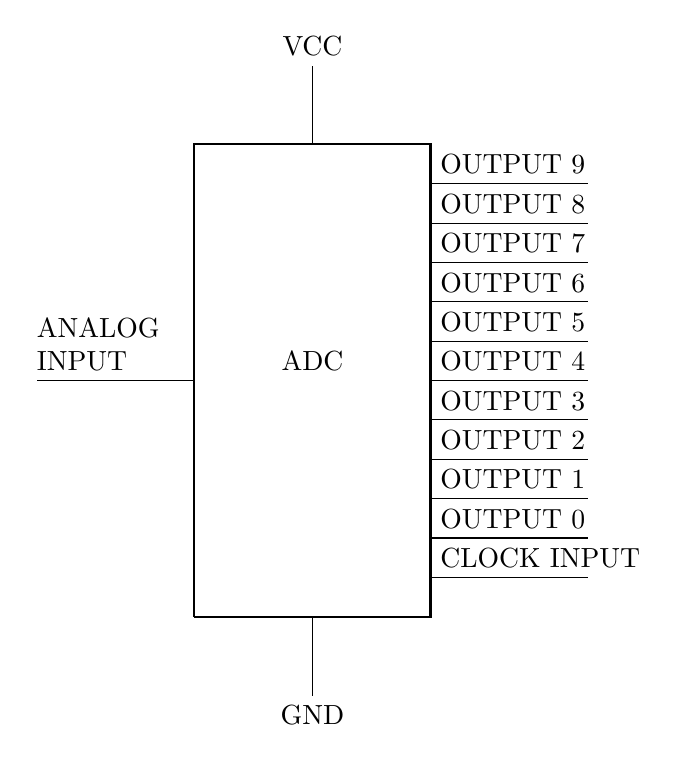
\begin{tikzpicture}
    \draw[thick] (0, 0) -- (0, 6.0) -- (3, 6.0) -- (3, 0) -- (0, 0);
    \draw (1.5, 3.00) node[right, above] {ADC};
    \draw (3, 0.5) node[anchor=south west] {CLOCK INPUT} -- (5, 0.5);
    \foreach \n/\y in {0/1.0, 1/1.5, 2/2.0, 3/2.5, 4/3.0, 5/3.5, 6/4.0, 7/4.5, 8/5.0, 9/5.5} {
      \draw (3, \y) node[anchor=south west] {OUTPUT \n} -- (5, \y);
    };
    \draw (0, 3.00)
    -- (-1, 3.00) node[left, above, text width=2cm] {ANALOG INPUT}
    -- (-2, 3.00);
    \draw (1.5, 6.0) -- (1.5, 7.0) node[right, above] {VCC};
    \draw (1.5, 0) -- (1.5, -1) node[right, below] {GND};
  \end{tikzpicture}
  \caption{Schematic depiction of the analog-to-digital converted (ADC.)}
  \label{fig:adc-schematics}
\end{figure}

The ADC takes some analog signal into the input (``ANALOG INPUT'') and encodes
it in each moment in time as the sequence of logical levels: ``HIGH'' (``1'')
and ``LOW'' (``0''.)  The ADC itself requires the power supply which is provided
through ``VCC'' and ``GND'' pins.  Also an ADC needs a clock signal (``CLOCK
INPUT'') -- on the value change on this input, ADC reads the current value of the
input analog signal and converts it to the digital representation on the
outputs.  Thus, the clock signal sets the frequency of ADC (or, to put it
differently, it controls the sampling frequency.)

\example{ Let's suppose we supplied 2.5V to the ADC input.  On the ``CLOCK
  INPUT'' toggle ADC forms a binary value ``1000000000'' on the outputs which
  represents the number $2^9 = 512$ -- that can be read in the program running on
  a micro-controller. }

The conversion of an analog signal to a digital form inside an ADC is done in
three steps:

\begin{enumerate}

\item \textbf{Sampling.}  During this step ADC takes samples from the input
  analog signal at regular intervals of time (see \ref{fig:adc-sampling}.)
  \index{Electronics!ADC!Sampling}

  \begin{figure}[h]
    \centering
    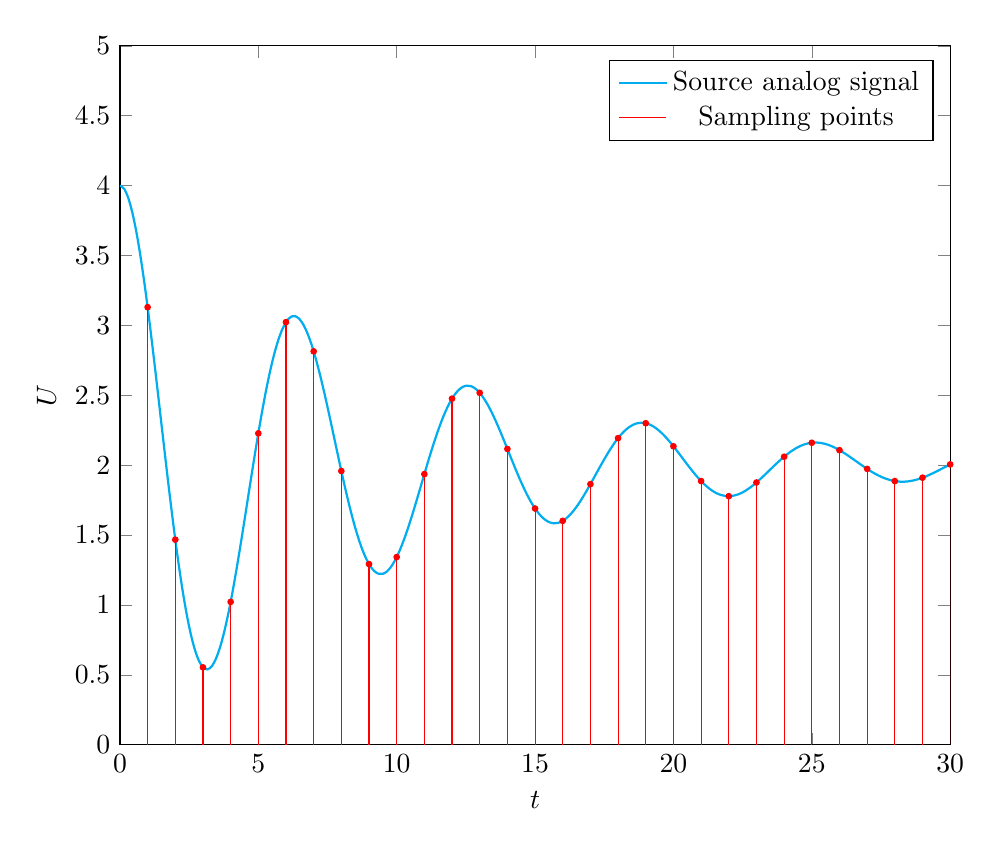
\begin{tikzpicture}
      [
        declare function={
          f(\x)=2 + exp(-\x/10)*( cos(deg(\x)) + sin(deg(\x))/10 ) * 2;
        }
      ]

      \begin{axis}[
          width = \textwidth,
	        xmin = 0, xmax = 30,
	        ymin = 0, ymax = 5.0,
          xlabel={$t$},
          ylabel={$U$}
        ]

	      \addplot[
		      domain = 0:30,
		      samples = 200,
		      smooth,
		      thick,
		      cyan
	      ] {
          2 + exp(-x/10)*( cos(deg(x)) + sin(deg(x))/10 ) * 2
        };

        \foreach \x [evaluate={\y=f(\x)}] in {1, 2, ..., 30} {
          \addplot[red]
          coordinates {
            (\x, 0) (\x, \y)
          };
          \addplot[red, mark = *, mark size=1.0pt]
          coordinates { (\x, \y) };
        };

        \legend{
	        Source analog signal,
          Sampling points
        }
	    \end{axis};
    \end{tikzpicture}
    \caption{Sampling.}
    \label{fig:adc-sampling-00}
  \end{figure}

  The frequency of those intervals is called \emph{sampling rate}.

    \begin{figure}[h]
    \centering
    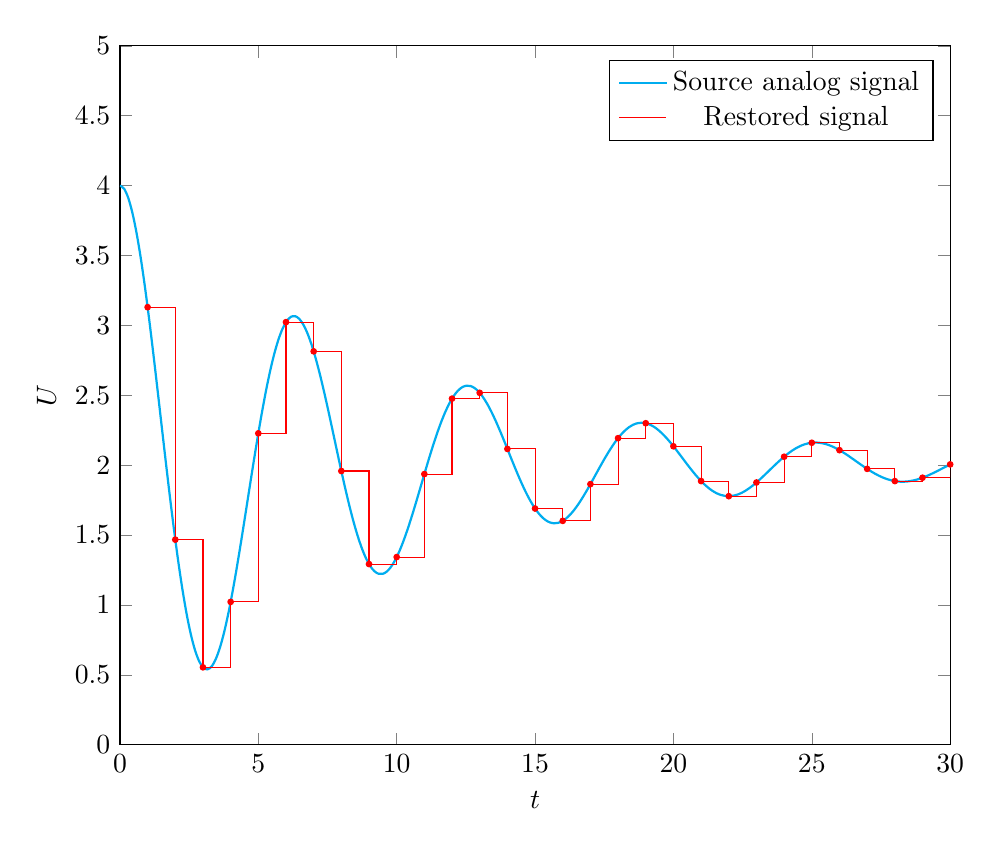
\begin{tikzpicture}
      [
        declare function={
          f(\x)=2 + exp(-\x/10)*( cos(deg(\x)) + sin(deg(\x))/10 ) * 2;
        }
      ]

      \begin{axis}[
          width = \textwidth,
	        xmin = 0, xmax = 30,
	        ymin = 0, ymax = 5.0,
          xlabel={$t$},
          ylabel={$U$},
        ]

	      \addplot[
		      domain = 0:30,
		      samples = 200,
		      smooth,
		      thick,
		      cyan
	      ] {
          2 + exp(-x/10)*( cos(deg(x)) + sin(deg(x))/10 ) * 2
        };

        \foreach \x [evaluate={\y=f(\x); \xnext=\x + 1; \ynext=f(\x + 1)}] in {1, 2, ..., 30} {
          \addplot[red]
          coordinates {
            (\x, \y) (\xnext, \y) (\xnext, \ynext)
          };
          \addplot[red, mark = *, mark size=1.0pt]
          coordinates { (\x, \y) };
        };

        \legend{
	        Source analog signal,
          Restored signal
        }
	    \end{axis}
    \end{tikzpicture}
    \caption{Rebuilding the source signal with recorded points.}
    \label{fig:adc-sampling-01}
  \end{figure}

    If we try to rebuild the source analog signal using the recorded points, we
    will get the graph similar to the one that is shown on
    fig. \ref{fig:adc-sampling-01}.  As we can see, some data got lost due to
    low sampling frequency -- that's why some parts of the graph were ``cut
    away.''

\item \textbf{Quantization.}  Acquired values are replaced with the closest
  values from the set of possible values -- \emph{quantization levels}.
  \index{Electronics!ADC!Quantization}

    \begin{figure}[h]
    \centering
    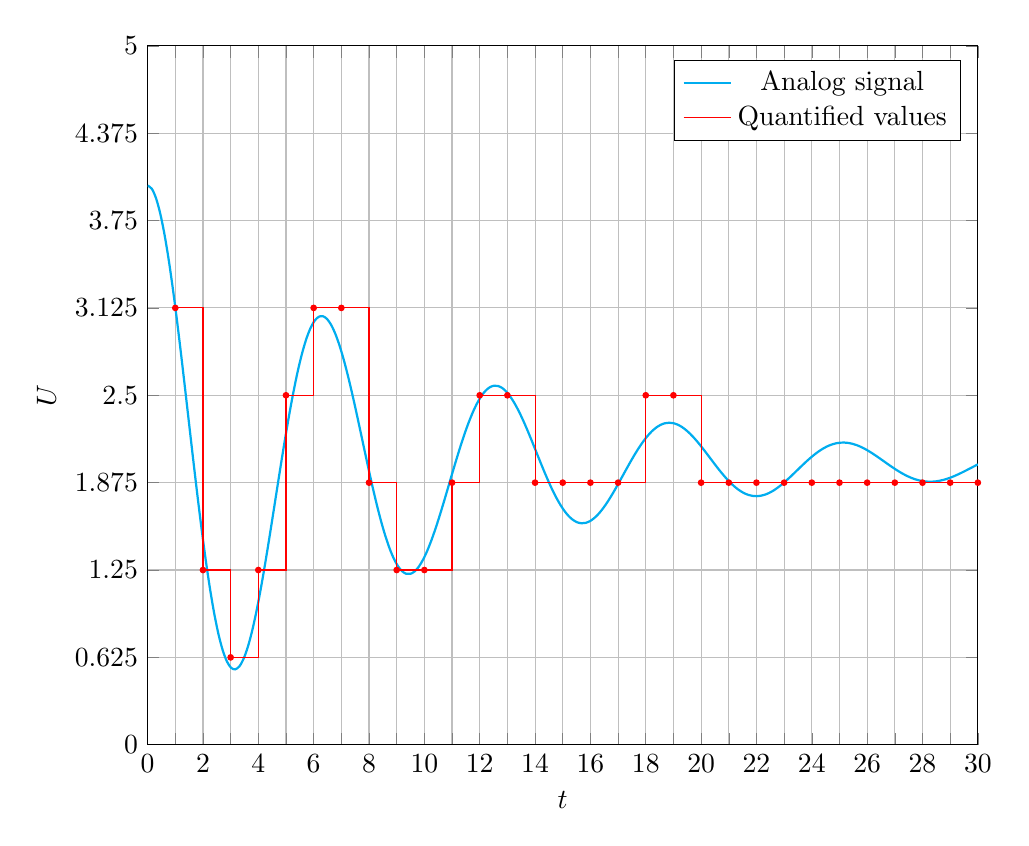
\begin{tikzpicture}
      [
        declare function={
          step=0.625;
          f(\x)=2 + exp(-\x/10)*( cos(deg(\x)) + sin(deg(\x))/10 ) * 2;
          q(\x)=mod(f(\x), step) == 0 ? f(\x) : ((int(round(f(\x) / step)) + 0) * step);
        }
      ]

      \begin{axis}[
          width = \textwidth,
	        xmin = 0, xmax = 30,
	        ymin = 0, ymax = 5.0,
          xlabel={$t$},
          ylabel={$U$},
          grid=both,
          grid style={line width=.2pt, draw=gray!10},
          major grid style={line width=.4pt,draw=gray!50},
          xtick distance = 1,
	        ytick distance = step,
          xtick = {0, 1, ..., 30},
          xticklabels={0,,2,,4,,6,,8,,10,,12,,14,,16,,18,,20,,22,,24,,26,,28,,30},
          /pgf/number format/precision=5
        ]

	      \addplot[
		      domain = 0:30,
		      samples = 200,
		      smooth,
		      thick,
		      cyan
	      ] {
          2 + exp(-x/10)*( cos(deg(x)) + sin(deg(x))/10 ) * 2
        };

        \foreach \x [evaluate={\y=q(\x); \xnext=\x + 1; \ynext=q(\x + 1)}] in {1, 2, ..., 30} {
          \addplot[red]
          coordinates {
            (\x, \y) (\xnext, \y) (\xnext, \ynext)
          };
          \addplot[red, mark = *, mark size=1.0pt]
          coordinates { (\x, \y) };
        };

        \legend{
	        Analog signal,
          Quantified values
        }
	    \end{axis}
    \end{tikzpicture}
    \caption{Quantization.}
    \label{fig:adc-quantization}
  \end{figure}

    The visual representation of the quantization process is shown on the
    fig. \ref{fig:adc-quantization}.  As we can see from the figure, in the
    quantified values we put points strictly on the cross-sections of the grid.
    The more horizontal lines in the grid, the closer we can set the value on
    the $y$ axis to the original value.

\item \textbf{Encoding.}  Binary codes are assigned to the resulting values (see
  \ref{fig:coding}.)
  \index{Electronics!ADC!Encoding}

  \begin{figure}[h]
    \centering
    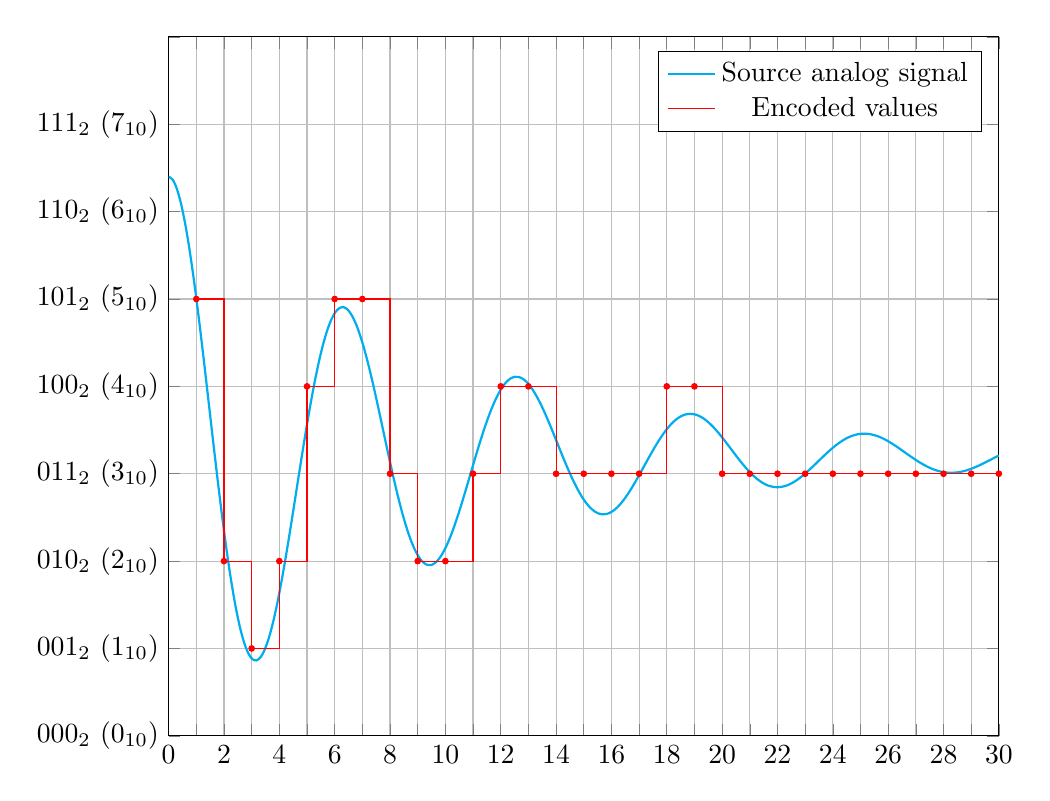
\begin{tikzpicture}
      [
        declare function={
          step=0.625;
          f(\x)=2 + exp(-\x/10)*( cos(deg(\x)) + sin(deg(\x))/10 ) * 2;
          q(\x)=mod(f(\x), step) == 0 ? f(\x) : ((int(round(f(\x) / step)) + 0) * step);
        }
      ]

      \begin{axis}[
          width = \textwidth,
	        xmin = 0, xmax = 30,
	        ymin = 0, ymax = 5.0,
          grid=both,
          grid style={line width=.2pt, draw=gray!10},
          major grid style={line width=.4pt,draw=gray!50},
          xtick distance = 1,
	        ytick distance = step,
          xtick = {0, 1, ..., 30},
          xticklabels={0,,2,,4,,6,,8,,10,,12,,14,,16,,18,,20,,22,,24,,26,,28,,30},
          /pgf/number format/precision=5,
          yticklabels={
            $000_2$ ($0_{10}$),
            $000_2$ ($0_{10}$),
            $001_2$ ($1_{10}$),
            $010_2$ ($2_{10}$),
            $011_2$ ($3_{10}$),
            $100_2$ ($4_{10}$),
            $101_2$ ($5_{10}$),
            $110_2$ ($6_{10}$),
            $111_2$ ($7_{10}$),
          }
        ]

	      \addplot[
		      domain = 0:30,
		      samples = 200,
		      smooth,
		      thick,
		      cyan
	      ] {
          2 + exp(-x/10)*( cos(deg(x)) + sin(deg(x))/10 ) * 2
        };

        \foreach \x [evaluate={\y=q(\x); \xnext=\x + 1; \ynext=q(\x + 1)}] in {1, 2, ..., 30} {
          \addplot[red]
          coordinates {
            (\x, \y) (\xnext, \y) (\xnext, \ynext)
          };
          \addplot[red, mark = *, mark size=1.0pt]
          coordinates { (\x, \y) };
        };

        \legend{
	        Source analog signal,
          Encoded values
        }
	    \end{axis};
    \end{tikzpicture}
    \caption{Encoding an analog signal in the binary form.}
    \label{fig:adc-encoding}
  \end{figure}

  An example of the 3-bit encoding is shown on the the
  fig. \ref{fig:adc-encoding}.

  The higher the sampling rate and the more quantization levels are available,
  the more precise is the analog-to-digital conversion.

\end{enumerate}

One of the main characteristics of the ADC is the \emph{resolution}.  It sets
the range for values that the ADC can output.

\index{Programming!Binary numeral system}

Computers are operating on the binary numeral system -- that is, the minimum
information storage unit, which is called \emph{bit}, can hold only one of the
two values: one or zero.

With two of such cells (bits) we can already store 4 combinations of the ones
and zeroes: 00, 01, 10, 11.  If we take 3 bits they will provide us with 8
combinations.  It's easy to see the pattern here: adding one additional bit
doubles the number of combinations.

We can calculate the number of combinations even easier: we don't have to put
ones and zeroes in imaginary ``cells'' and count them.  We can use the following
formula instead:

\begin{equation}
  \mbox{Number of combinations} = 2^{\mbox{n}}
\end{equation}

Where \texttt{n} is the number of available bits for storing some value.

For example, if we take 8 bits to store some data it will give us $2^8 = 256$
combinations of ones and zeroes.

Let's take a look on the graph on fig. \ref{fig:coding}: for encoding the values
we are using three bits -- thus, the ADC described by this graph, has the
resolution of 3 bits.  That is, the number of quantization levels is equal to
$2^3 = 8$.

But we should not forget that the counting in the computer world is usually
starts from zero, and the case when all the bits are set to zero, is the one of
the possible values.  Let's suppose we have 8 bits and we have set them to ones:
$11111111_2$.  If we convert this value into the decimal form we will get:

\begin{equation}
  11111111_2 = (2^7 * 1) + \mbox{...} + (2^2 * 1) + (2^1 * 1) + (2^0 * 1) = 255_{10}
\end{equation}

Thus we can see that the maximum positive value for 8 bits is equal to 255.

From that it follows that if we take 10 bits to store some information, we can
encode 1024 combinations of ones and zeroes, because $2^{10} = 1024$.  But the
maximum positive value will be equal to 1023.  Thus in Arduino the ADC has the
10-bits resolution.

Also there's a different system that is called \emph{digital-to-analog
converter} (DAC) which performs the inverse function of ADC -- that is, converts
a digital signal to an analog signal.

The use of ADCs and DACs is very widespread: it is used in audio/video cards, in
displays, in various audio equipment, in measurement devices (such as
oscilloscopes) and in many more areas.

We will discuss the DAC in the chapter \ref{chapter:pwm} titles ``Pulse-width
modulation.''

\subsection{Operation of ADC using temperature measurement as an example}
\label{subsection:adc-temperature-example}

Suppose we have to measure the air temperature outside our window to plot a
graph afterwards.  For this task we have to organize a table in the following
format:

\begin{table}[h]
  \centering
  \begin{tabular}{p{3cm}|p{4cm}}
    Measurement time & Temperature \\
    \hline \hline
    06:00 & -5 \\
    \hline
    12:00 & -7 \\
    \hline
    18:00 & -8 \\
    \hline
    00:00 & -10 \\
    \hline
  \end{tabular}
  \caption{An example data about air temperature variation.}
  \label{table:adc-temperature-data-example-1}
\end{table}

The measurements are taken in uniform time intervals and for each measurement
the timestamp and the air temperature is written down.

How can we improve the quality of our data?  There are two main parameters that
we can adjust:

\begin{itemize}
\item We can increase the \emph{frequency of the measurements}: if we perform
  measurements more often, it will allow us to register the dynamics of changes
  more precise.
\item We can increase the \emph{accuracy of measurements}: if we perform more
  accurate measurements, it will allow us to register smaller changes in the
  values.
\end{itemize}

An example of more frequent measurements (once in 3 hours) is shown in table
\ref{table:adc-temperature-data-example-2}.

\begin{table}[h]
  \centering
  \begin{tabular}{p{3cm}|p{4cm}}
    Measurement time & Temperature \\
    \hline \hline
    06:00 & -5 \\
    \hline
    09:00 & -4 \\
    \hline
    12:00 & -7 \\
    \hline
    15:00 & -8 \\
    \hline
    18:00 & -8 \\
    \hline
    21:00 & -9 \\
    \hline
    00:00 & -10 \\
    \hline
  \end{tabular}
  \caption{An example data about air temperature variation with more frequent
    measurements.}
  \label{table:adc-temperature-data-example-2}
\end{table}

If we also increase the accuracy of measurements, we will get the table similar
to подобную \ref{table:adc-temperature-data-example-3}.

\begin{table}[h]
  \centering
  \begin{tabular}{p{3cm}|p{4cm}}
    Measurement time & Temperature \\
    \hline \hline
    06:00 & -5.2 \\
    \hline
    09:00 & -4.1 \\
    \hline
    12:00 & -7.2 \\
    \hline
    15:00 & -8.5 \\
    \hline
    18:00 & -8.9 \\
    \hline
    21:00 & -9.0 \\
    \hline
    00:00 & -10.7 \\
    \hline
  \end{tabular}
  \caption{An example data about air temperature variation with more frequent
    and more accurate measurements.}
  \label{table:adc-temperature-data-example-3}
\end{table}

In case of ADC, the increase in the frequency of measurements is called the
increase in sampling rate.  In this regard, the increase in recording accuracy
is called the increase in resolution of the converter.

In case of ADC a computer measures the voltage on the analog input (for example,
from a temperature sensor.)  After that the analog-to-digital conversion takes
place where each voltage value is assigned some digital value from the available
range, set by the converter resolution.

As the result, for example, in case of -5.2 degrees Celsius on a thermometer, a
computer may read it as the value of 1.3 Volts.  Further, a digital value of
$01110101_2$ ($117_{10}$) is assigned to this value (see
\ref{table:adc-temperature-data-example-4}.

\begin{table}[h]
  \centering
  \begin{tabular}{p{3cm}|p{4cm}|p{4cm}}
    Measurement time & Temperature & The ADC output value \\
    \hline \hline
    06:00 & -5.2  & 117 \\
    \hline
    09:00 & -4.1  & 121 \\
    \hline
    12:00 & -7.2  & 109 \\
    \hline
    15:00 & -8.5  & 104 \\
    \hline
    18:00 & -8.9  & 103 \\
    \hline
    21:00 & -9.0  & 102 \\
    \hline
    00:00 & -10.7 & 95 \\
    \hline
  \end{tabular}
  \caption{An example of data with binary encoding.}
  \label{table:adc-temperature-data-example-4}
\end{table}

%% TODO: Describe 8-bit music in detail here as an example of ADC.

\end{document}

